\documentclass{article}
\usepackage[utf8]{inputenc}
\usepackage{graphicx}


\title{ ASSIGNMENT 10}
\author{Srinitha Beerelly}
\date{8 JAN , 2021} 

\begin{document}

\maketitle
\section{Problem Statement :}

Consider the given circuit\\


\begin{center}
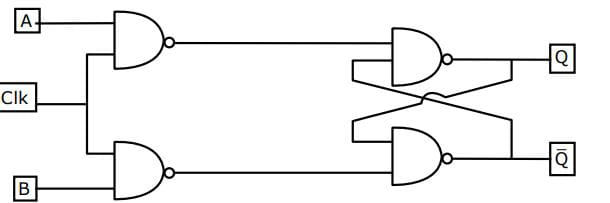
\includegraphics[width=200,height=50]{CIRCUIT.jpeg}
\end{center}


in this circuit, the race around \\
(A) does not occur\\
(B) occurs when CLK=0\\
(C) occurs when CLK=1 and A=B=1\\
(D) occurs when CLK=1 and A=B=0\\

\maketitle
\section{Explanation:}
\begin{center}
Q_n_e_x_t = \overline{\overline{A.CLK}.{\overline{Q}}}\\
=A.CLK + Q\\
\overline{Q}_n_e_x_t = B.CLK + \overline{Q}\\
If  CLK = 1 and  A = B =1\\
then  Q_n_e_x_t = 1\\
\overline{Q}_n_e_x_t =1\\
then  no  race  around\\
If CLK = 1 and A = B =0\\
then  Q_n_e_x_t = Q\\
\overline{Q}_n_e_x_t = \overline{Q}\\
then no race around\\
Thus race around does not occur in the circuit
\end{center}

\maketitle
\section{Answer}

the answer to the given question is (A)

\\
\begin{center}
\underline{To Be Noted} : Race around is applicable only for J-K flip flop when CLK = 1 and A=B=1. But the given circuit is S-R flip flop so no race around occurs.
\end{center}                         

\maketitle
\section{STATE TRANSITION TABLE}

\begin{center}
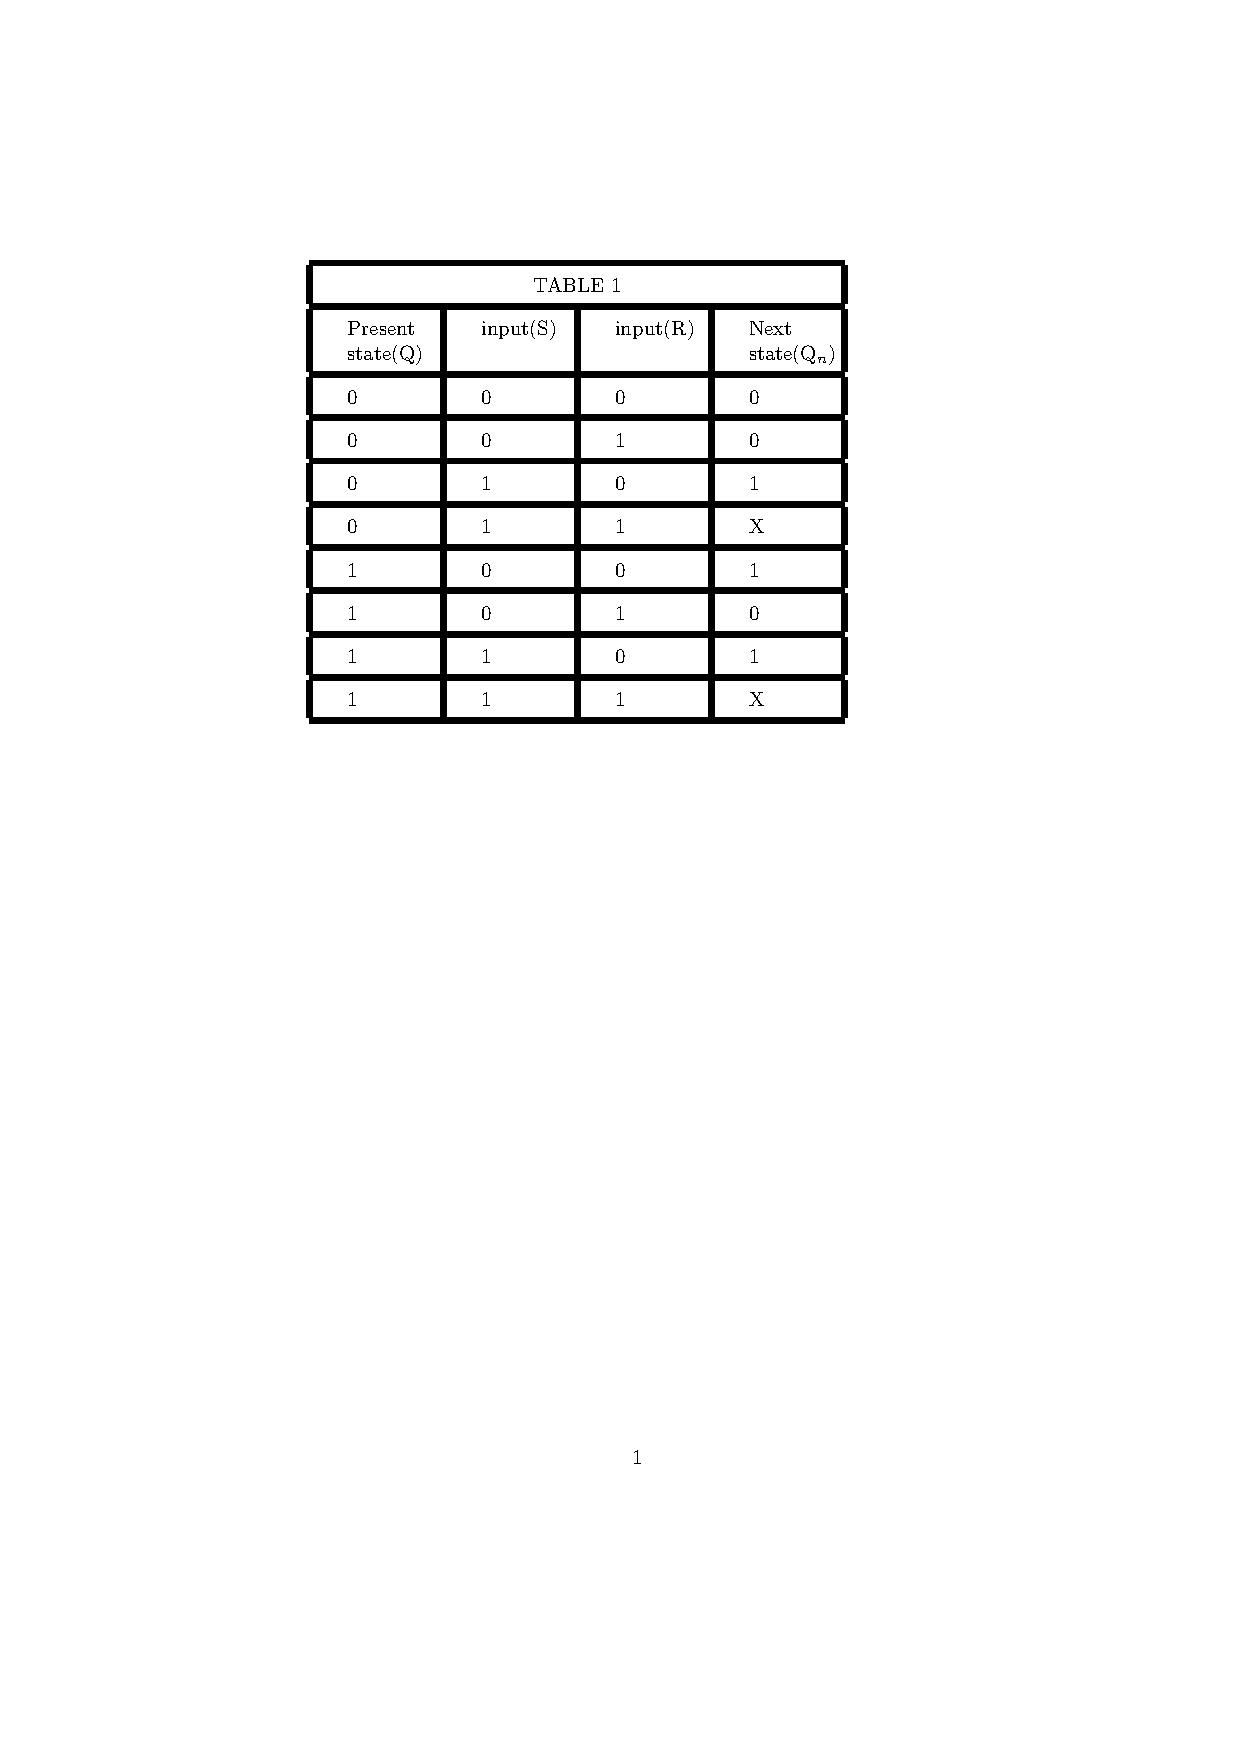
\includegraphics[width=400,height=400]{STATE_TRANSITION_TABLE.pdf}
\end{center}


\end{document}